\section{Tracks}
\label{sec:ch6_tracks}

\subsection{Reconstruction}

A track is reconstructed by fitting the trajectory of a charged particle to measurements in the ID.
Its momentum and charge are determined from the curvature in the magnetic field, while its position near the beam line is used to associate it with a production vertex.
Track reconstruction is performed in the following stages~\cite{ATLAS2017DenseTracking}:
\begin{enumerate}
    \item \textbf{Space-point formation.} Signals in neighbouring channels of a silicon sensor are grouped into clusters. The coordinates provided by Pixel clusters and SCT clusters are converted into three-dimensional space points.
    \item \textbf{Seeding and track finding.} Combinations of space points are used to form track seeds. These seeds are extended through the silicon layers with a combinatorial Kalman filter, which is used to refine the track parameters.
    \item \textbf{Ambiguity resolution.} Track candidates are ranked based on their fit quality, assigned clusters and other criteria. And candidates that share the same clusters are marked as "shared hits". At last the low-quality candidates that fail the track-quality or hit-sharing requirements are rejected to suppress duplicate and fake tracks.
    \item \textbf{TRT extension.} Tracks are extended with additional TRT hits. The extended track is retained if its quality score is higher than that of the original track reconstructed using only pixel and SCT hits.
\end{enumerate}

\subsection{Track parameters and quality}

The fitted trajectory is specified by five parameters as illustrated in Figure~\ref{fig:ch6_track_parameters}:
\begin{itemize}
    \item $d_0$: distance in the $x-y$ plane between the beam line and the nearest point on the track (the perigee point).
    \item $z_0$: distance from the reference $z=0$ plane to the perigee point.
    \item $\phi$ and $\theta$: the azimuthal and polar angles of the momentum.
    \item $q/p$: the electric charge divided by the momentum magnitude.
\end{itemize}

%介绍写后面会出现的impact-parameter，例如D- significance和Z0sintheta

\begin{figure}[htbp]
    \centering
    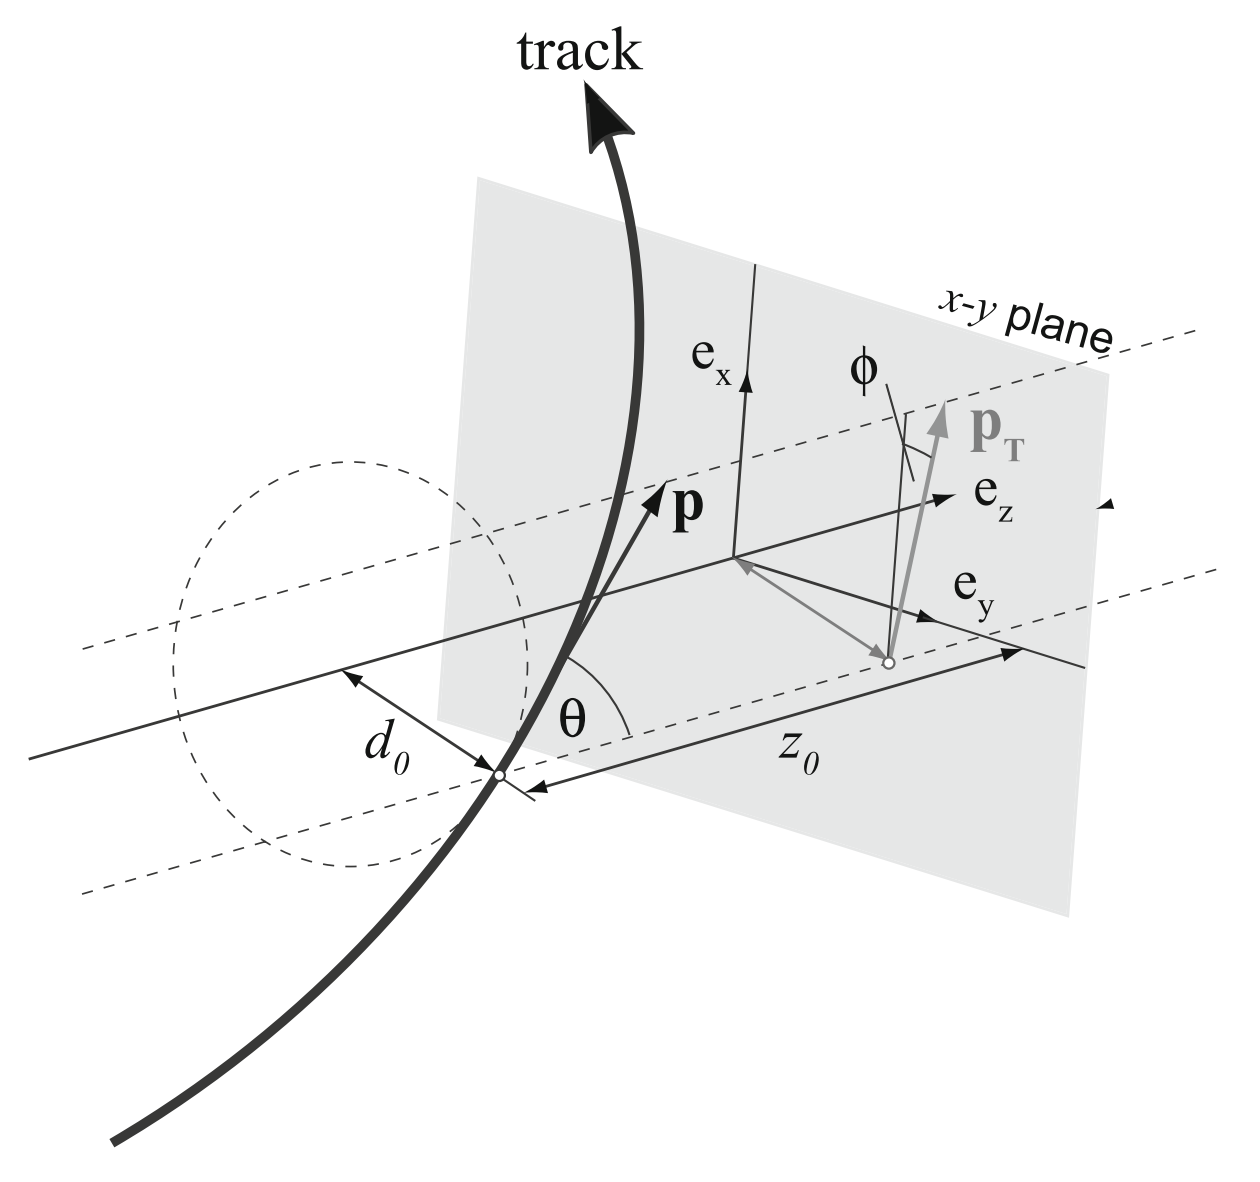
\includegraphics[width=0.58\textwidth]{output/ch6/figures/track_parameters.png}
    \caption[Geometry of the Track parameters]{Geometry of the Track parameters. The grey plane represents the reference $z=0$ plane~\cite{ATLAS2025SoftwareComputing}.}
    \label{fig:ch6_track_parameters}
\end{figure}
